\section{AST rewriting}
\label{sect:method:ast_rewrite}
\begin{myDefinition}
\label{definition:normalisation}
The process of \textbf{normalisation} is defined as the process of translating the
whole or parts of an XQuery abstract syntax tree into an XQuery Core abstract
syntax tree, as described in section \ref{sect:theory:xquery:XQcore}.
\end{myDefinition}

\begin{myDefinition}
\label{definition:denormalised}
An abstract syntax tree is said to be \textbf{denormalised} if it has not yet
been normalised through a process of normalisation.
\end{myDefinition}

The basic abstract syntax tree produced by the XQFT Parser (see section
\ref{sect:theory:xqftparser}) is in a denormalised form. As explained in
section \ref{sect:theory:xquery:XQcore} on page
\pageref{sect:theory:xquery:XQcore}, normalisation has the benefit of
simplification without loss of expressiveness or semantics, and thus
simplifying the task of translating the syntax tree.

Based on findings in section \ref{sect:theory:xquery:Flwor} regarding the
structure of FLWOR expressions, it was briefly mentioned that complex FLWOR
expressions could be transformed into semantically equivalent and simpler
representations. A question was also posed -- \emph{could it be
benefitial to rewrite complex FLWOR expressions into a simpler form}? We will
now attempt to answer this question.

\subsection{Normalising FLWOR expressions}
A denormalised XQuery syntax tree may contain nodes such \texttt{for}-clause expressions with several variable
declarations and assignments as can be seen in figure \ref{tree:ast:flwor_rewrite1}. Such an expression could be
normalised to several nested FLWOR expressions, as shown in figure \ref{tree:ast:flwor_rewrite2}, as defined by
the mapping rules in figures \ref{figure:xquery:flwor_mapping_rule},
\ref{figure:xquery:where_mapping_rule},
\ref{figure:xquery:orderby_mapping_rule}, and
\ref{figure:xquery:return_mapping_rule}.

Here, the method in section \ref{sect:theory:xquery:core:rewriting_flwor} has
been applied to the example tree in figure \ref{figure:ast_rewrite:flwor1},
and the result can be seen in figure \ref{figure:ast_rewrite:flwor3}. The
corresponding hypothetical source code for the denormalised and normalised trees
can be seen in figure \ref{figure:ast_rewrite:flwor_src}.

\begin{figure}[!h]
	\centering
	\mbox{
		\subfigure[Step 1: original denormalised syntax tree]{
			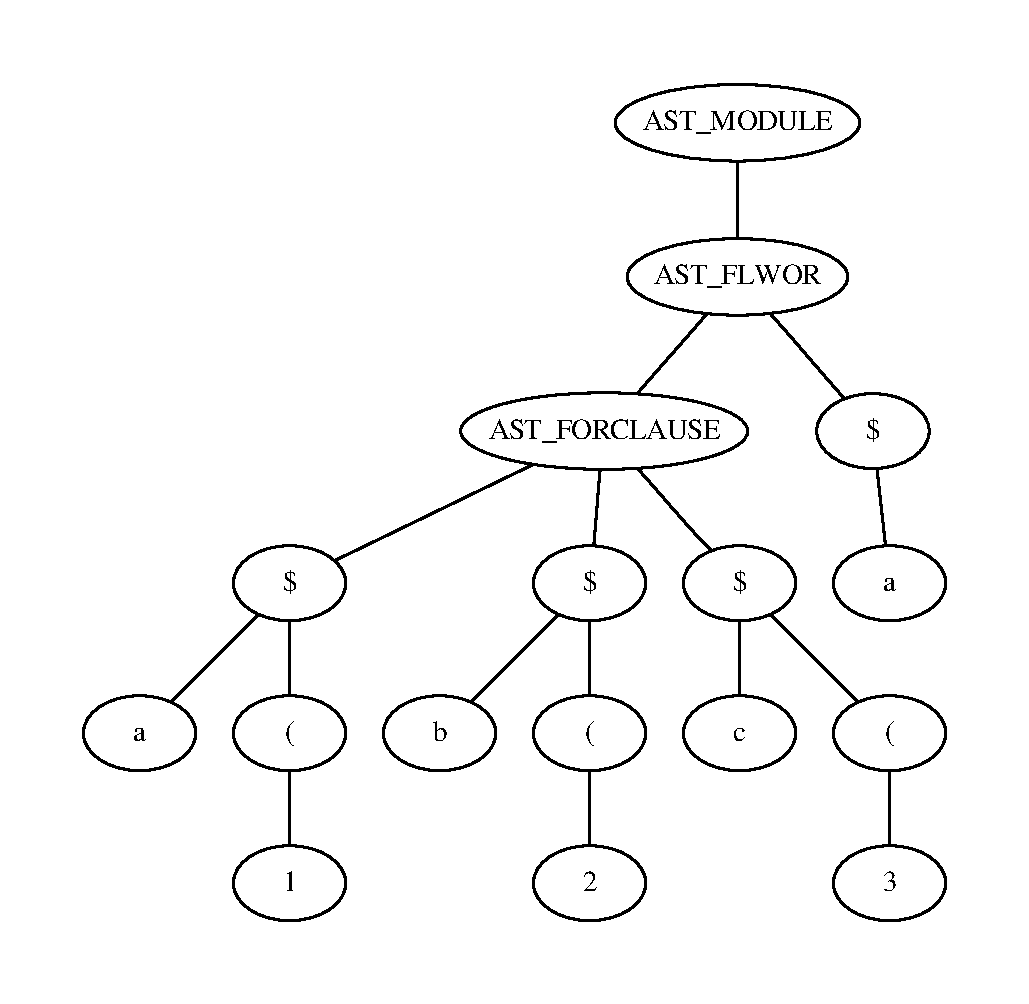
\includegraphics[scale=0.22]{img/graphs/flwor_rewrite_p1} 
			\label{figure:ast_rewrite:flwor1}
		}
		\quad
		\subfigure[Step 2: partly normalised tree]{
			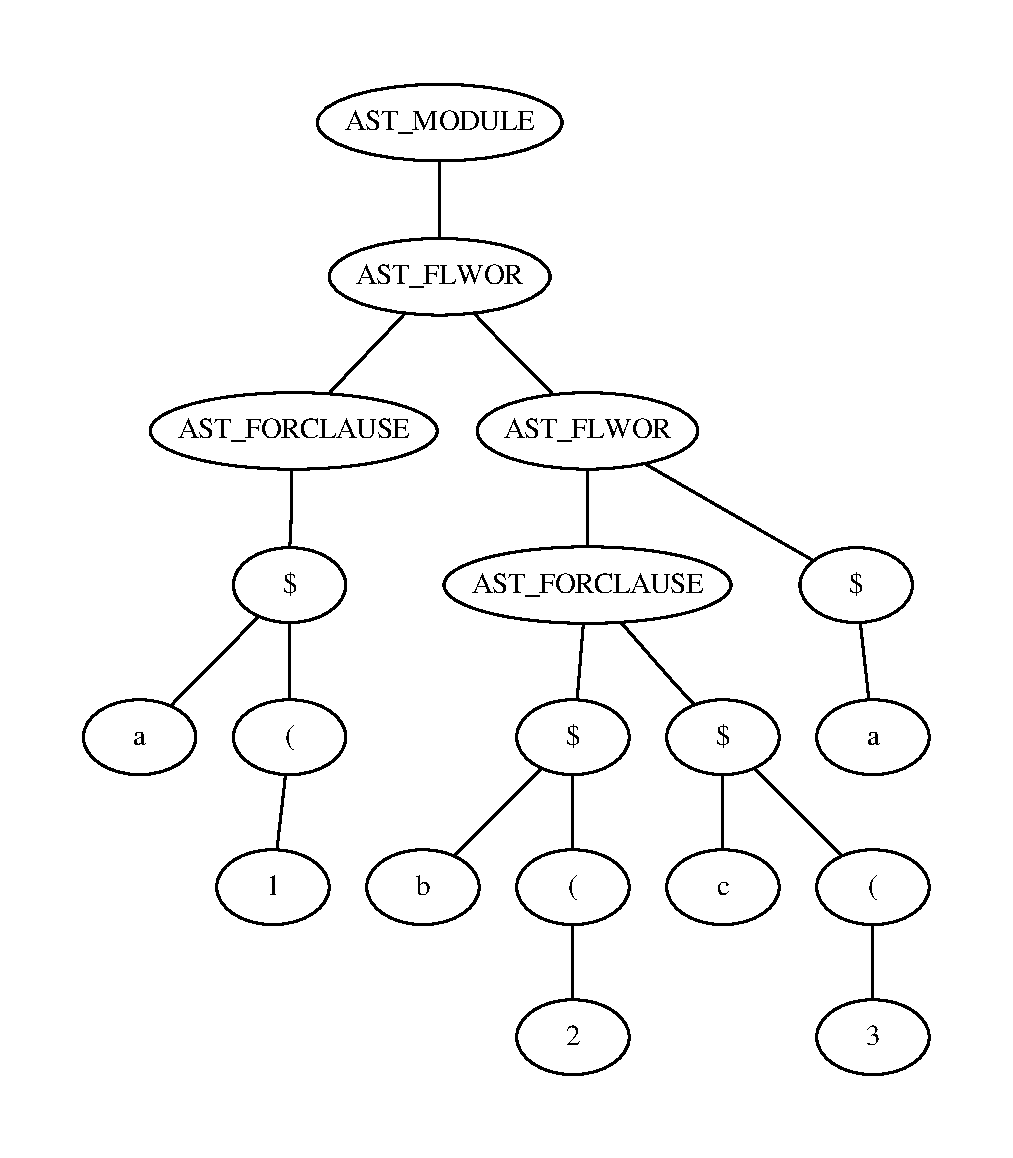
\includegraphics[scale=0.22]{img/graphs/flwor_rewrite_p2} 
			\label{figure:ast_rewrite:flwor2}
		}
		\quad
		\subfigure[Step 3: fully normalised tree]{
			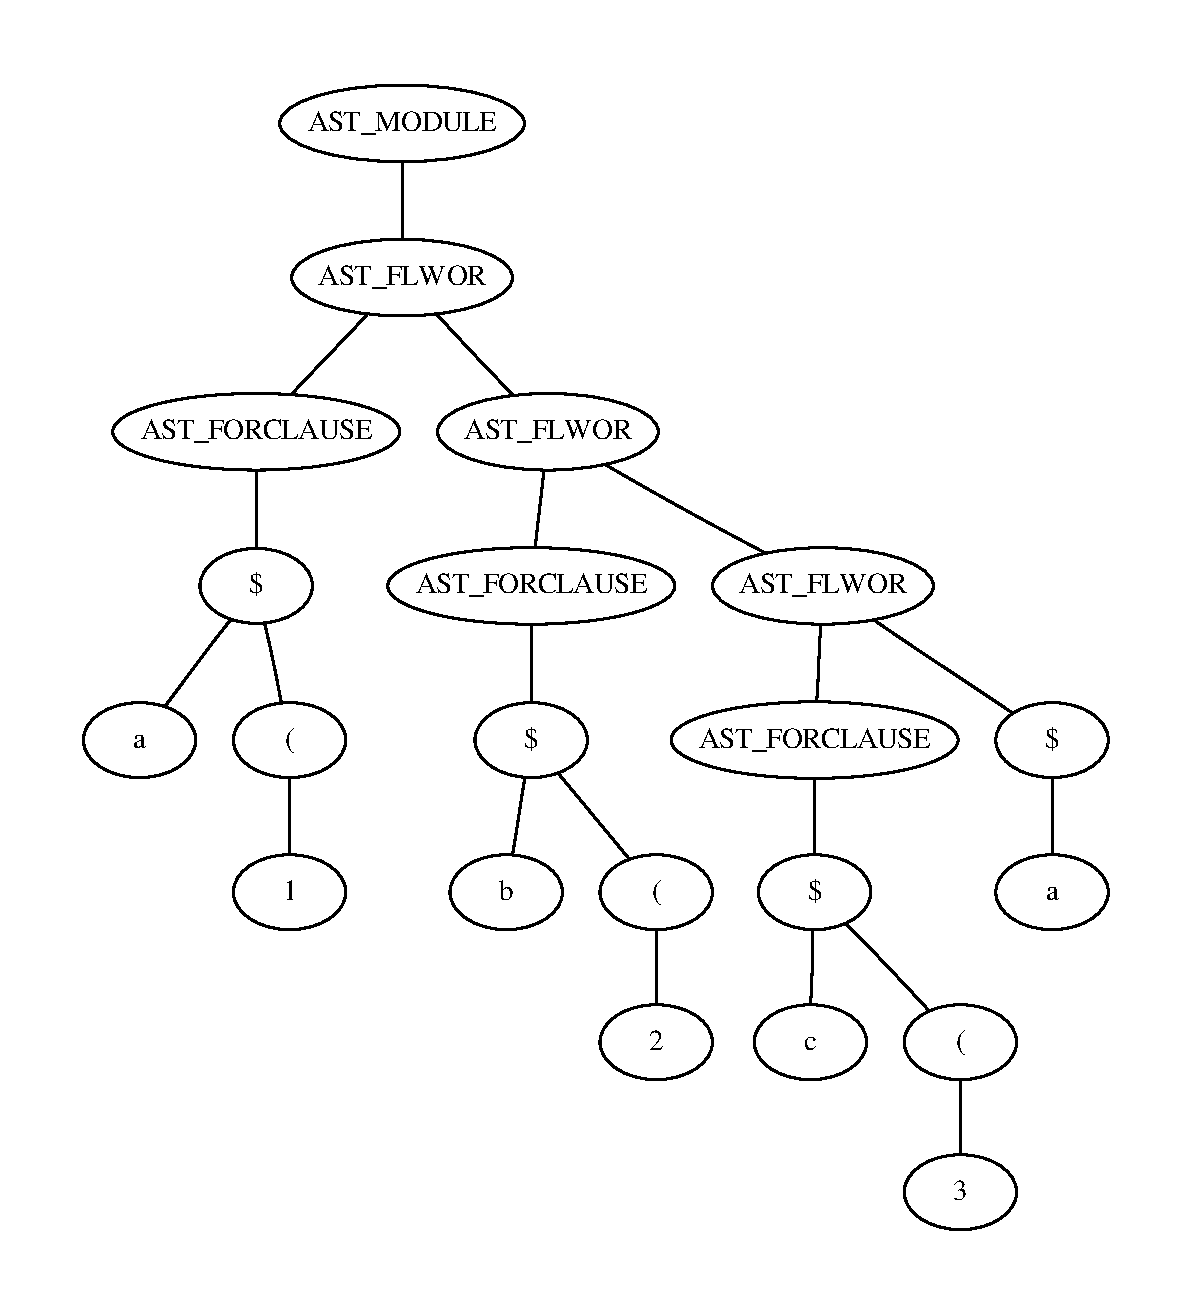
\includegraphics[scale=0.22]{img/graphs/flwor_rewrite_p3} 
			\label{figure:ast_rewrite:flwor3}
		}
	}
	\caption{Normalisation steps of FLWOR expression with multiple \texttt{for}-clauses}
\end{figure}

\begin{figure}[!h]
	\centering
	\mbox{
		\subfigure[]{
			\mbox {
				
				 \begin{minipage}{0.3\textwidth}
				 	\verbatiminput{graph_queries/flwor_rewrite_p1.xq}
 				 \end{minipage}
			}
			\label{figure:ast_rewrite:flwor1_src}
		}
		\quad
		\subfigure[]{
			\mbox{
				 \begin{minipage}{0.3\textwidth}
				 	\verbatiminput{graph_queries/flwor_rewrite_p3.xq}
 				 \end{minipage}
			}
			\label{figure:ast_rewrite:flwor2_src}
		}
	}
	\caption{Hypothetical source code corresponding to the trees in figures
		\ref{figure:ast_rewrite:flwor1} and \ref{figure:ast_rewrite:flwor3}}
	\label{figure:ast_rewrite:flwor_src}
\end{figure}

Considering these trees, we can assert the following:
\begin{enumerate}
  \item Multiple nested FLWOR constructs with a single \texttt{for/let}-clause
  and a single variable binding maintains the semantics of a single FLWOR with
  multiple \texttt{for/let}-clauses and variable bindings
  \item A FLWOR construct with a single \texttt{for/let}-clause and a single
  variable binding is easier to parse than a FLWOR construct with multiple
  \texttt{for/let}-clauses and bindings because it is known that there is only
  one \texttt{for/let}-clause with a variable binding, and there is no need to
  look for others within the same FLWOR construct
\end{enumerate}

Based on these findings, it is natural to conclude that normalisation of FLWOR
expressions is benefitial for the sake of simplicity in the tree parsing
process. Normalisation may be attained by executing a specialised
\textit{rewrite visitor} on the syntax tree, which will be described in
chapter \ref{chapter:implementation}.
